% ===========================================================================
% Section IV-C -- Multi-Load Adaptive Thresholding
% Owner: Member 3
% ===========================================================================
\begin{figure*}[!t]
\centering
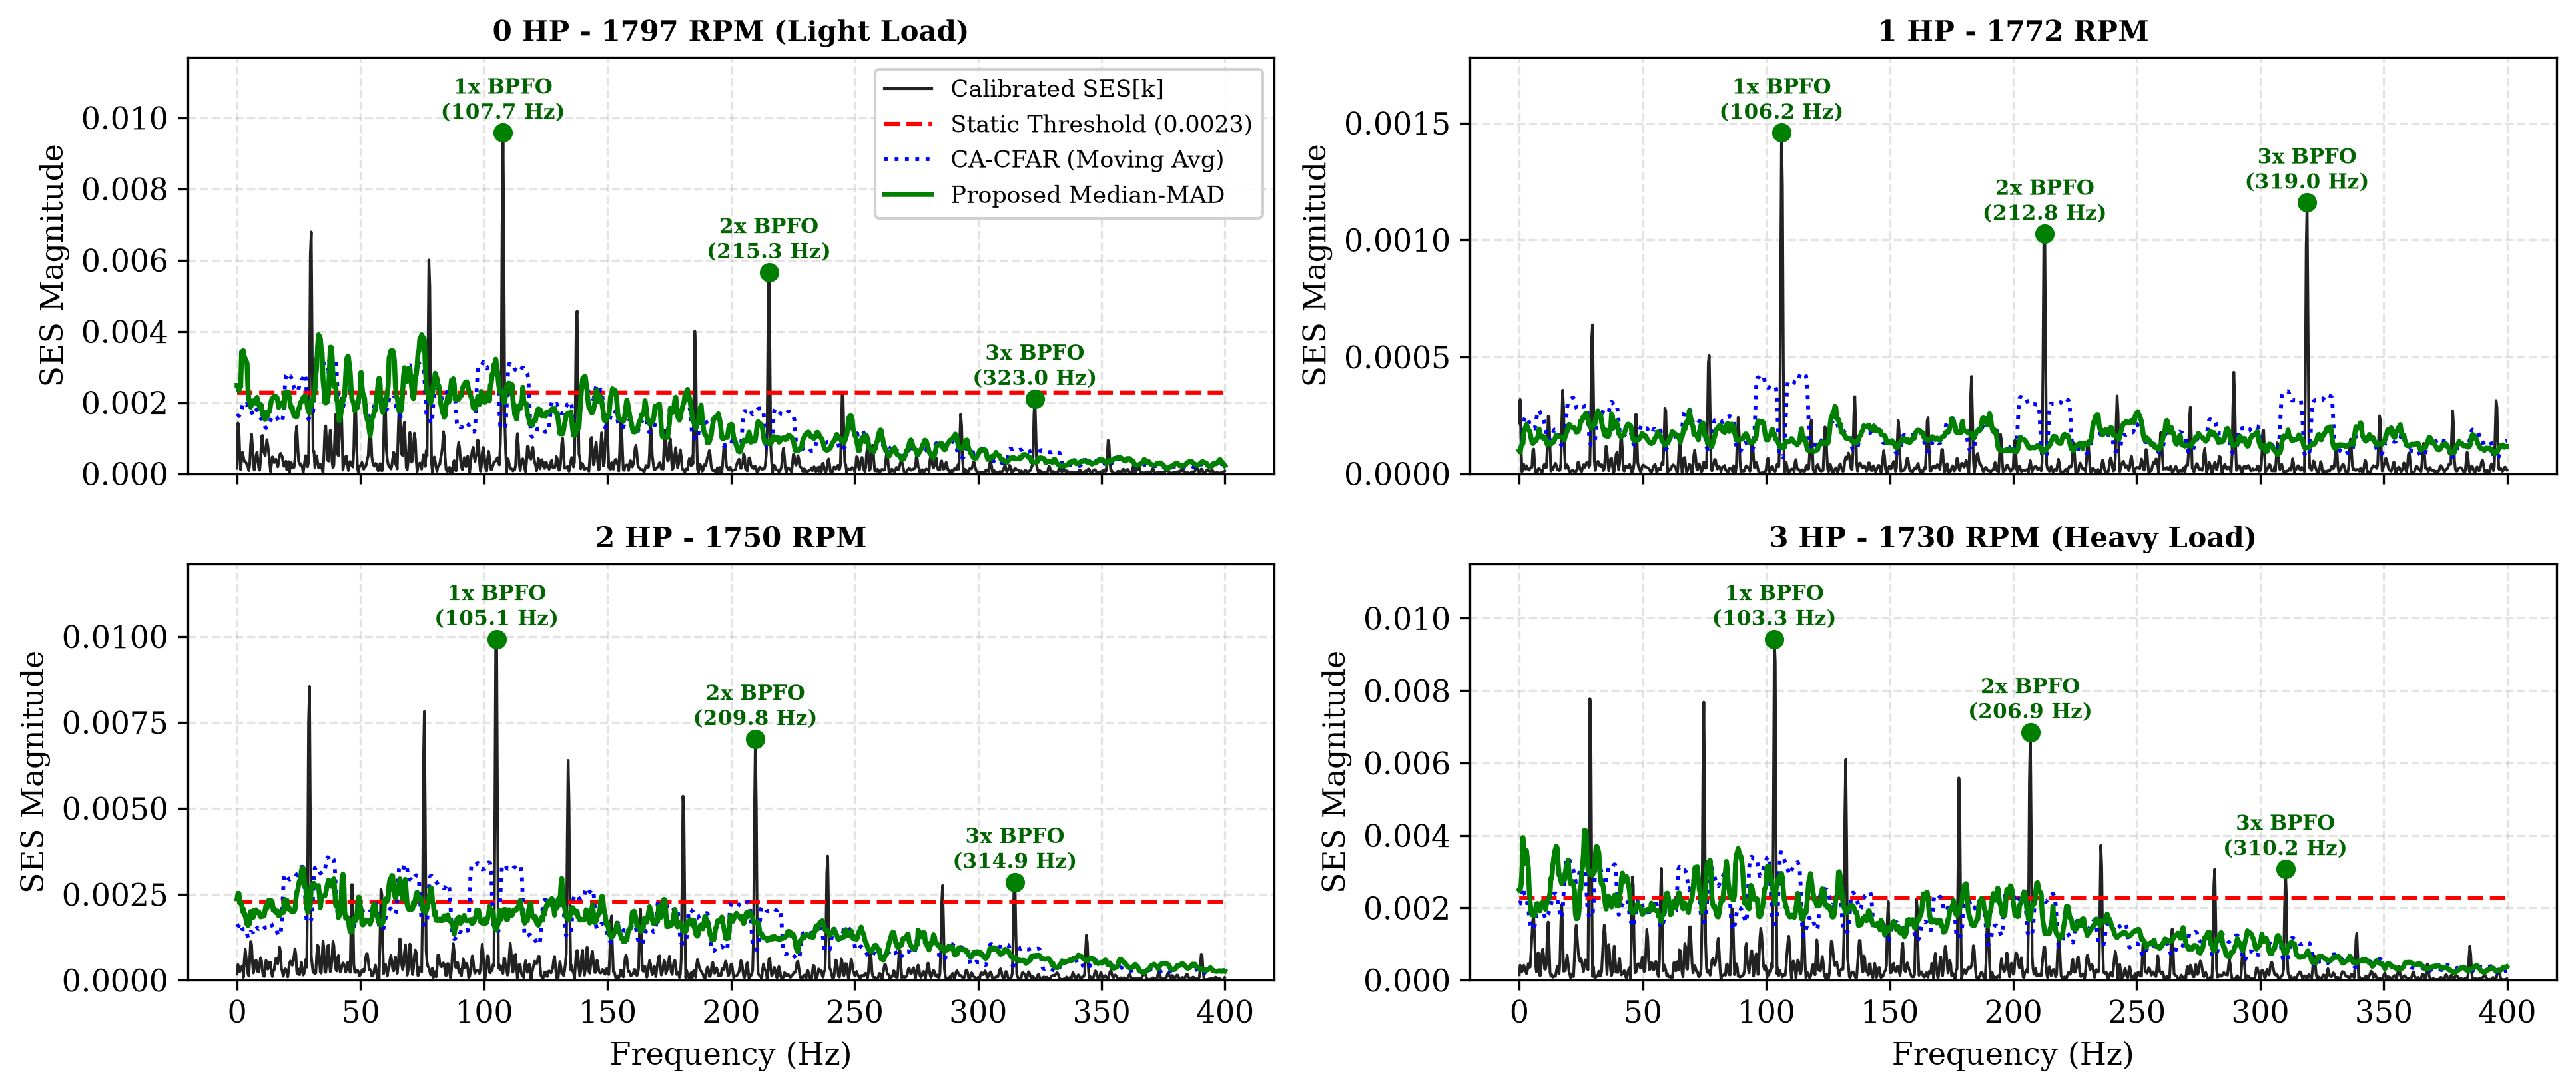
\includegraphics[width=0.88\textwidth]{Fig3_MultiLoad_SES_Thresholding.png}
\caption{Calibrated SES and comparative thresholding at four motor loads for
the outer-race $7$~mil record. The static threshold is calibrated once on the
$0$~HP reference ($T_{\text{static}}=0.00228$); it marks two of the three BPFO
harmonics in the $0$~HP panel, none in the $1$~HP panel and all three in the
$2$ and $3$~HP panels. CA-CFAR ($3.7$--$8.6\%$) and Median--MAD
($3.6$--$7.4\%$) crossings follow the load-dependent floor and flag all three
BPFO harmonics in every panel.}
\label{fig:ses}
\end{figure*}

\subsection{Multi-Load Adaptive Thresholding}
Fig.~\ref{fig:ses} shows the calibrated SES and the three thresholds for an
outer-race defect at the four motor loads of Table~\ref{tab:kinematics}. The
fixed level held at $0.00228$ is not scale-invariant: its crossing share swings
from $0\%$ to $2\%$ between panels and its per-segment detection rate ranges
from $40$ to $80\%$ with spreads up to $55$ points, so whether a harmonic
clears it depends on the segment rather than on the load. Both adaptive rules
follow the load-dependent floor and flag the $1\times$, $2\times$ and
$3\times$ BPFO harmonics in every panel; Table~\ref{tab:benchmark} measures the
difference quantitatively.
